\subsection{Referenzszenario aktualisierte Kostensätze}

\subsubsection{Kenngrößen Szenario}

\captionof{table}{\label{table_4_kenngrößen_scenario} Basiskenngrößen Szenario 4}
\begin{center}
	\begin{tabularx}{\textwidth}{X | X } Kenngröße & Wert \\
	\hline
	Anzahl Untersuchungsgebiete & \num{154} \\
	Summe Streckenkilometer & \SI{13490.0}{\km}
	\end{tabularx}
\end{center}

\subsubsection{Kenngrößen Untersuchungsgebiete}
\captionof{table}{\label{table_4_kenngrößen_untersuchungsgebiete} Kenngrößen Untersuchungsgebiete Szenario 4}
\begin{center}
	\begin{tabularx}{\textwidth}{X | X | X} Traktion & Anzahl & Kilometer \\
	\hline
            electrification & \num{26} &  \SI{8.0}{\km}\\
            efuel & \num{0} &  \SI{0}{\km}\\
            battery & \num{102} &  \SI{91.0}{\km}\\
            optimised electrification & \num{26} &  \SI{103.0}{\km}\\
            diesel & \num{0} &  \SI{0}{\km}\\
            h2 & \num{0} &  \SI{0}{\km}\\
            no calculated cost & \num{0} &  \SI{0}{\km}\\
    	\end{tabularx}
\end{center}

\captionof{table}{\label{table_4_kenngrößen_untersuchungsgebiete_no_optimised} Kenngrößen Untersuchungsgebiete (Optimierte Elektrifizierung aufgeteilt) Szenario 4}
\begin{center}
	\begin{tabularx}{\textwidth}{X | X | X} Traktion & Anzahl & Kilometer \\
	\hline
            electrification & \num{26} &  \SI{3305.0}{\km}\\
            efuel & \num{0} &  \SI{0}{\km}\\
            battery & \num{102} &  \SI{10185.0}{\km}\\
            optimised electrification & \num{26} &  \SI{0}{\km}\\
            diesel & \num{0} &  \SI{0}{\km}\\
            h2 & \num{0} &  \SI{0}{\km}\\
            no calculated cost & \num{0} &  \SI{0}{\km}\\
    	\end{tabularx}
\end{center}
In dieser Tabelle wurden die Infrastrukturkilometer der Untersuchungsgebiete, bei denen die optimierte Elektrifizierung am wirtschaftlichsten war, auf die Traktionen Elektrifizierung und Batterie aufgeteilt (je nachdem, bei welchem Teiluntersuchungsgebiet welche Traktion am wirtschaftlichsten war)

\begin{center}
	\begin{figure}[!h]
	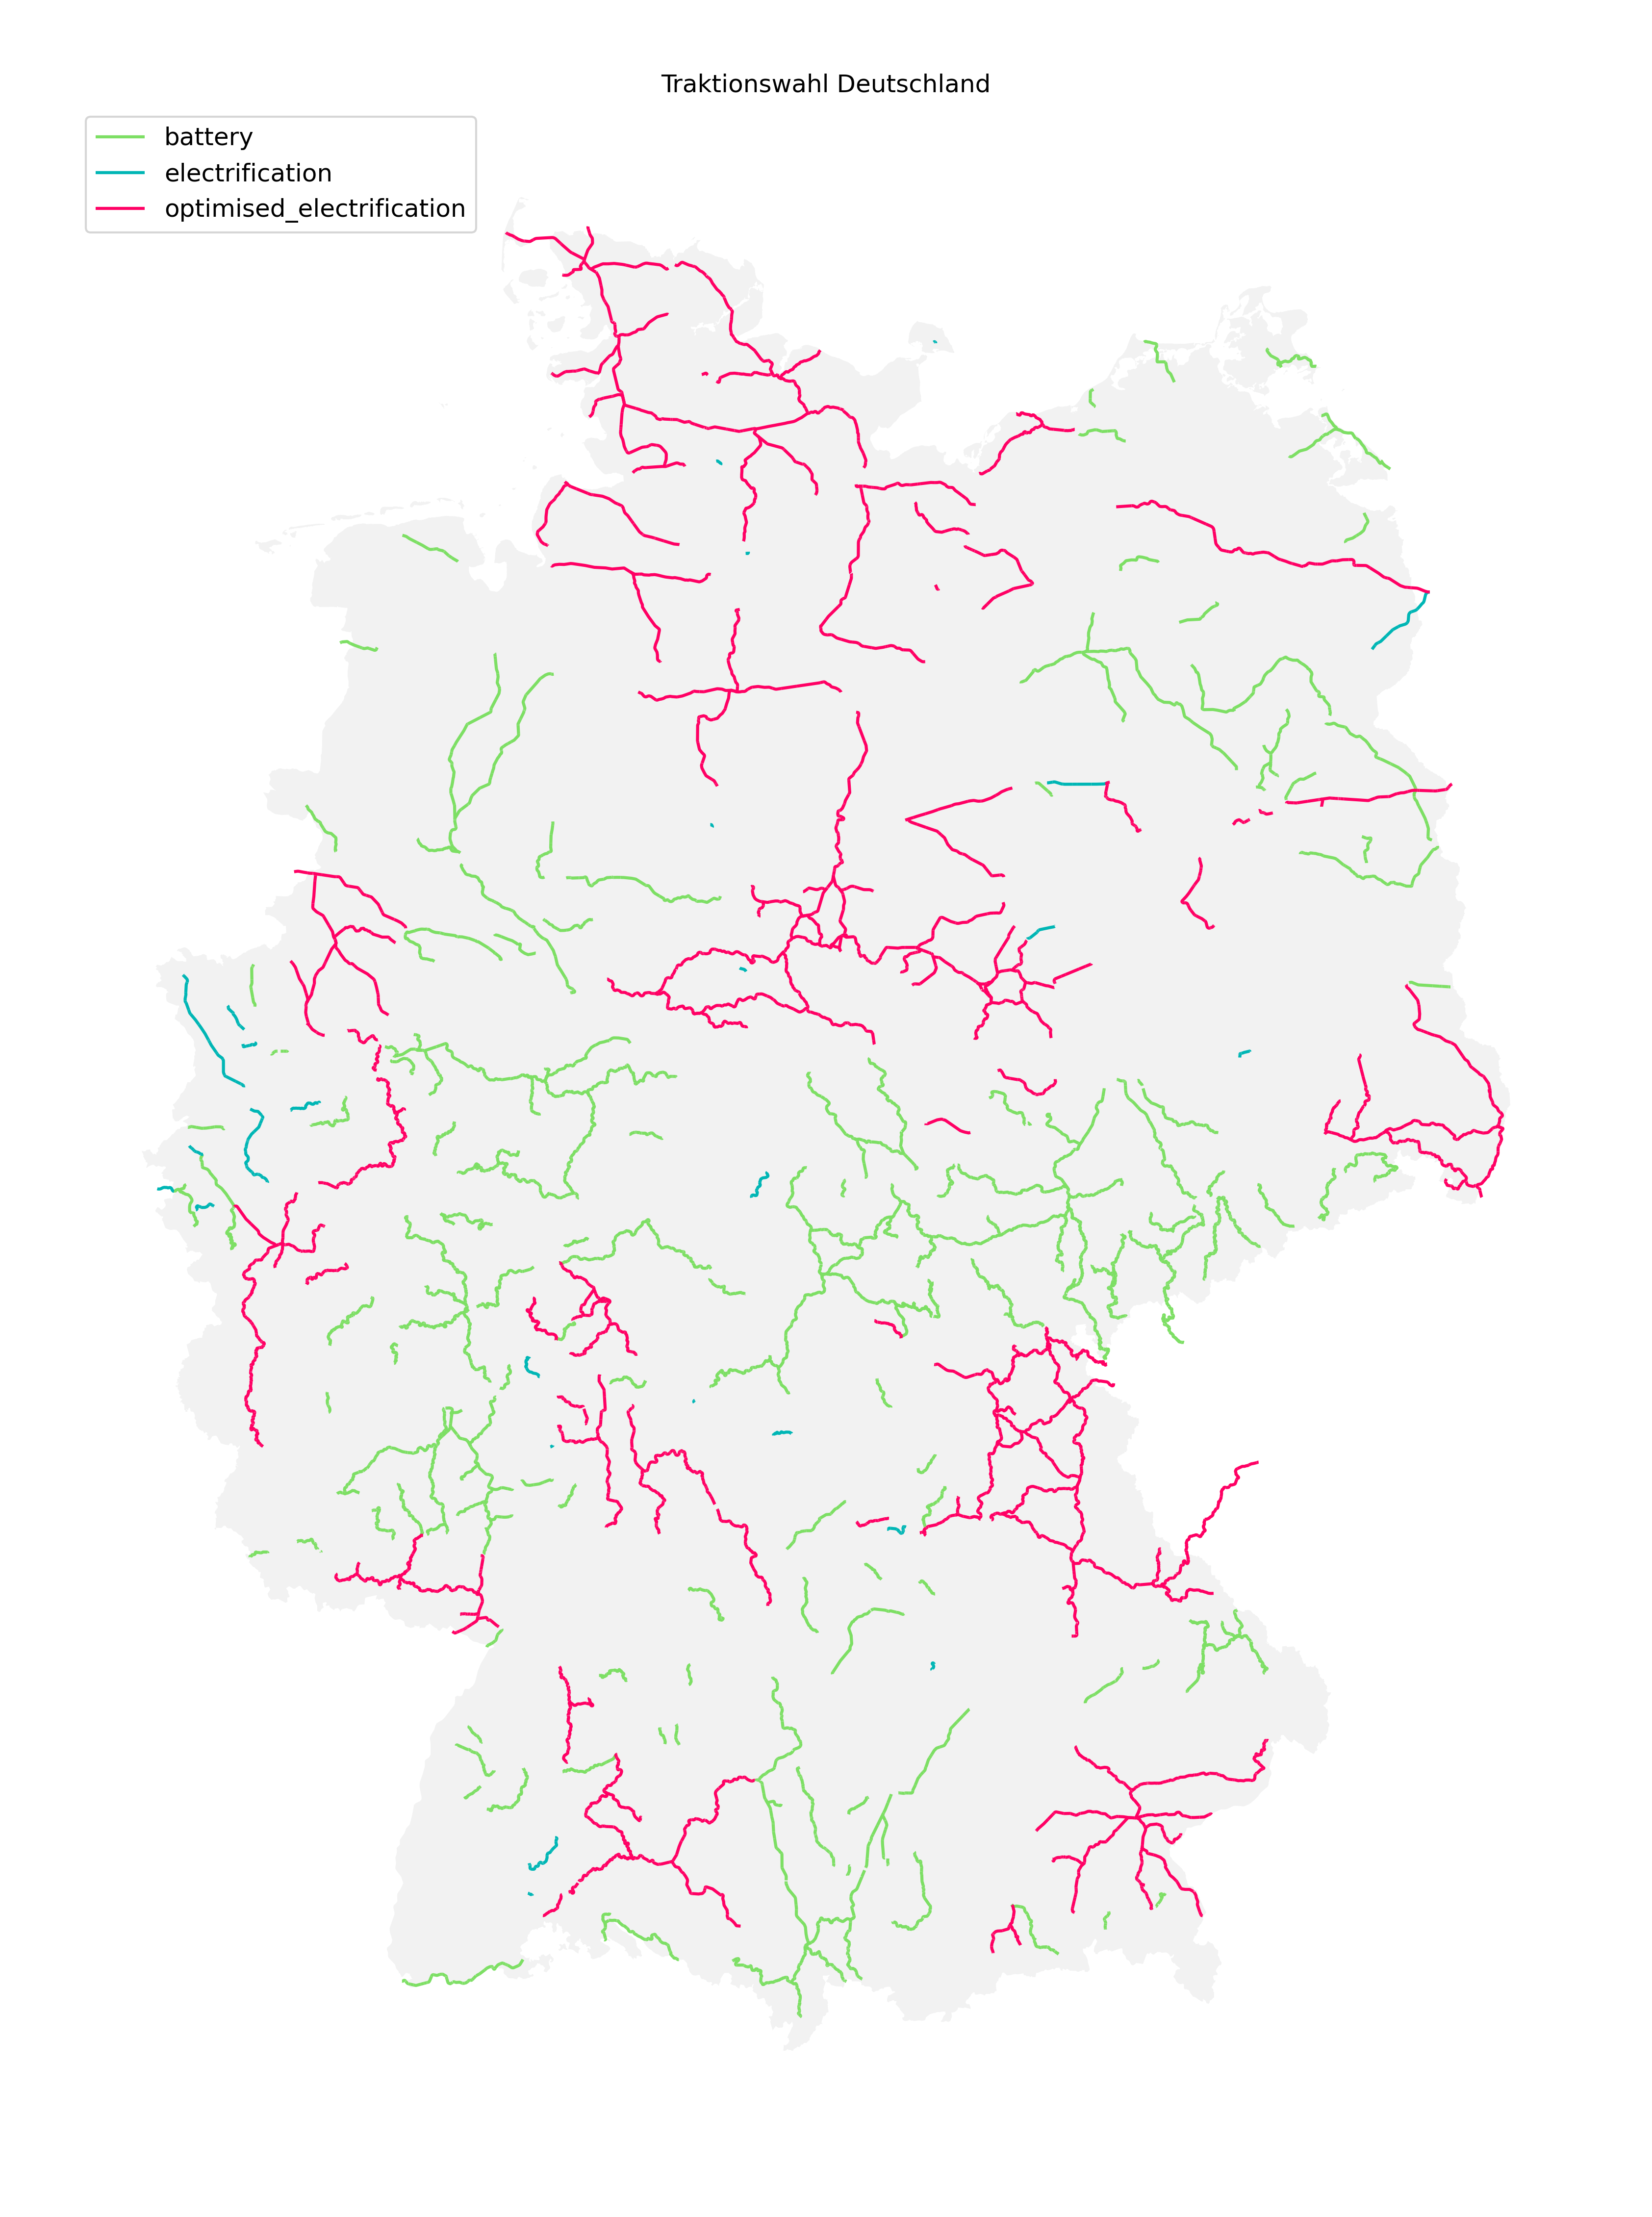
\includegraphics[height=0.8\paperheight]{../report_scenarios/s_4/files/deutschland_map.png}
	\caption{\label{fig_s_4_d_map} Karte Deutschland bevorzugte Traktion Untersuchungsgebiete Szenario 4 (Darstellung: PyCharm)}
	\end{figure}
\end{center}